\documentclass[14pt]{extarticle}


\usepackage{amsmath, amssymb, amsthm, amsfonts, mathrsfs}
\usepackage{times, flexisym, mdframed, xcolor}
\usepackage{ulem,multicol}
\usepackage{mathtools}
\usepackage{tikz}
\usepackage{hyperref}
\usepackage{graphicx}
\usepackage{fancyhdr}
\usepackage{tikz-cd}%   Margins
% \usepackage[left=1in,right=1in, top=2in, bottom=2in]{geometry}
\usepackage[paperwidth= 20in,paperheight=12in,left=.25in,right=12in, top=.25in, bottom=.25in]{geometry}
%

\usepackage{draculatheme}
\graphicspath{ {./images/} }
\parindent0pt
\begin{document}

Floating point arithmetic. The standard formula for computing the roots of a quadratic $a x^{2}+b x+c=0$ :
$$
x=\frac{-b \pm \sqrt{b^{2}-4 a c}}{2 a}
$$
is known to have problems computing the smaller root numerically if $b^{2}$ is much larger than $|a c|$. Explain the cause of the cause of this problem; propose a method for avoiding this problem.
%%%%%%%%%%%%%%%%%%%%%%%%%%%%%%%%%%%%%%%%%%%%%%%%%%%%%%%%%%%%%%%%%%%%%%%%%%%%%%%%%%%%%%%%%%%%%%%%%%%%%%%%%%%%%%%%%%%%%%%%
\newpage
%%%%%%%%%%%%%%%%%%%%%%%%%%%%%%%%%%%%%%%%%%%%%%%%%%%%%%%%%%%%%%%%%%%%%%%%%%%%%%%%%%%%%%%%%%%%%%%%%%%%%%%%%%%%%%%%%%%%%%%%
Solution of nonlinear equations. Carry out two steps of the secant method for solving $x-\cos x=0$ starting with $x_{0}=0$ and $x_{1}=1$. What rate of convergence is expected, and under what conditions is this rate of convergence obtained?
%%%%%%%%%%%%%%%%%%%%%%%%%%%%%%%%%%%%%%%%%%%%%%%%%%%%%%%%%%%%%%%%%%%%%%%%%%%%%%%%%%%%%%%%%%%%%%%%%%%%%%%%%%%%%%%%%%%%%%%%
\newpage
%%%%%%%%%%%%%%%%%%%%%%%%%%%%%%%%%%%%%%%%%%%%%%%%%%%%%%%%%%%%%%%%%%%%%%%%%%%%%%%%%%%%%%%%%%%%%%%%%%%%%%%%%%%%%%%%%%%%%%%%
Interpolation and approximation. Using equally spaced interpolation points is known to result in Runge's phenomenon for the function $f(x)=1 /\left(1+x^{2}\right)$ interpolated over $[-5,+5]$. What is this phenomenon? Can the use of a different set of interpolation points prevent this phenomenon? If so, explain how?
%%%%%%%%%%%%%%%%%%%%%%%%%%%%%%%%%%%%%%%%%%%%%%%%%%%%%%%%%%%%%%%%%%%%%%%%%%%%%%%%%%%%%%%%%%%%%%%%%%%%%%%%%%%%%%%%%%%%%%%%
\newpage
%%%%%%%%%%%%%%%%%%%%%%%%%%%%%%%%%%%%%%%%%%%%%%%%%%%%%%%%%%%%%%%%%%%%%%%%%%%%%%%%%%%%%%%%%%%%%%%%%%%%%%%%%%%%%%%%%%%%%%%%
 Numerical integration. Use Simpson's method with five function evaluations to obtain an estimate of $\int_{0}^{1} e^{x} /(1+x) d x$. What is the asymptotic order of the error of composite Simpson's method with $2 n+1$ function evaluations? Give an example of a method that has an asymptotically faster rate of convergence than Simpson's method as the number of function evaluations goes to infinity.
%%%%%%%%%%%%%%%%%%%%%%%%%%%%%%%%%%%%%%%%%%%%%%%%%%%%%%%%%%%%%%%%%%%%%%%%%%%%%%%%%%%%%%%%%%%%%%%%%%%%%%%%%%%%%%%%%%%%%%%%
\newpage
%%%%%%%%%%%%%%%%%%%%%%%%%%%%%%%%%%%%%%%%%%%%%%%%%%%%%%%%%%%%%%%%%%%%%%%%%%%%%%%%%%%%%%%%%%%%%%%%%%%%%%%%%%%%%%%%%%%%%%%%
Multistep methods. Consider the general multistep method
$$
y_{n+1}=\sum_{j=0}^{p} a_{j} y_{n-j}+h \sum_{j=-1}^{p} b_{j} f\left(t_{n-j}, y_{n-j}\right) .
$$
In order to prove convergence of a particular order for this method we need two basic conditions: a stability condition, and a consistency condition. Give these conditions. Use them to determine if, and with what order, the leap-frog method converges:
$$
y_{n+1}=y_{n-1}+2 h f\left(t_{n}, y_{n}\right) .
$$
%%%%%%%%%%%%%%%%%%%%%%%%%%%%%%%%%%%%%%%%%%%%%%%%%%%%%%%%%%%%%%%%%%%%%%%%%%%%%%%%%%%%%%%%%%%%%%%%%%%%%%%%%%%%%%%%%%%%%%%%
\newpage
%%%%%%%%%%%%%%%%%%%%%%%%%%%%%%%%%%%%%%%%%%%%%%%%%%%%%%%%%%%%%%%%%%%%%%%%%%%%%%%%%%%%%%%%%%%%%%%%%%%%%%%%%%%%%%%%%%%%%%%%
Runge-Kutta methods. Show that Heun's method
$$
\begin{aligned}
&\mathbf{z}_{n+1}=\mathbf{y}_{n}+h \mathbf{f}\left(t_{n}, \mathbf{y}_{n}\right), \\
&\mathbf{y}_{n+1}=\mathbf{y}_{n}+\frac{1}{2} h\left[\mathbf{f}\left(t_{n}, \mathbf{y}_{n}\right)+\mathbf{f}\left(t_{n+1}, \mathbf{z}_{n+1}\right)\right]
\end{aligned}
$$
has a local truncation error of $\mathcal{O}\left(h^{3}\right)$. What is its asymptotic global truncation error in the form $\mathcal{O}\left(h^{m}\right)$ ?
%%%%%%%%%%%%%%%%%%%%%%%%%%%%%%%%%%%%%%%%%%%%%%%%%%%%%%%%%%%%%%%%%%%%%%%%%%%%%%%%%%%%%%%%%%%%%%%%%%%%%%%%%%%%%%%%%%%%%%%%
\newpage
%%%%%%%%%%%%%%%%%%%%%%%%%%%%%%%%%%%%%%%%%%%%%%%%%%%%%%%%%%%%%%%%%%%%%%%%%%%%%%%%%%%%%%%%%%%%%%%%%%%%%%%%%%%%%%%%%%%%%%%%
LU factorization and linear systems. The perturbation theorem for linear systems states that if $A \boldsymbol{x}=\boldsymbol{b},(A+E) \widehat{\boldsymbol{x}}=\boldsymbol{b}+\boldsymbol{d}$, and $\left\|A^{-1}\right\|\|E\|<$ 1 , then
$$
\frac{\|\hat{x}-\boldsymbol{x}\|}{\|\boldsymbol{x}\|} \leq \frac{\kappa(A)}{1-\kappa(A)(\|E\| /\|A\|)}\left[\frac{\|E\|}{\|A\|}+\frac{\|d\|}{\|\boldsymbol{b}\|}\right]
$$
where $\kappa(A)=\left\|A^{-1}\right\|\|A\|$ is the condition number. Using this, how many digits of accuracy are expected in the computed solution $\widehat{x}$ given that the matrix $A$ and right-hand side $b$ are known to 5 digits, but $\kappa(A) \approx 10^{3}$ ? The backward error theory for $L U$ factorization by Wilkinson shows that the computed solution $\hat{x}$ of a system $A x=b$ exactly satisfies $(A+E) \widehat{x}=\boldsymbol{b}$ where $\|E\|_{\infty} \leq 3 \mathbf{u}\left(\|A\|_{\infty}+\|\widehat{L}\|_{\infty}\|\widehat{U}\|_{\infty}\right)$ where $\widehat{L}$ and $\widehat{U}$ are the computed $L$ and $U$ factors in the $L U$ factorization. If $\|\widehat{L}\|_{\infty}\|\widehat{U}\|_{\infty} /\|A\|_{\infty}$ is modest (say $\approx 10$ ), give an estimate for the relative error $\|\widehat{x}-x\|_{\infty} /\|x\|_{\infty}$ in terms of $\kappa(A)$ in the $\infty$-norm. 4. Least squares and $Q R$ factorization. What is a QR factorization of a matrix? Describe two different ways of computing the QR factorization of an $m \times n$ matrix. Explain how to use a QR factorization of a matrix to solve a least squares problem $\min _{\mathbf{x}}\|A \mathbf{x}-\mathbf{b}\|_{2}$.
%%%%%%%%%%%%%%%%%%%%%%%%%%%%%%%%%%%%%%%%%%%%%%%%%%%%%%%%%%%%%%%%%%%%%%%%%%%%%%%%%%%%%%%%%%%%%%%%%%%%%%%%%%%%%%%%%%%%%%%%
\newpage
%%%%%%%%%%%%%%%%%%%%%%%%%%%%%%%%%%%%%%%%%%%%%%%%%%%%%%%%%%%%%%%%%%%%%%%%%%%%%%%%%%%%%%%%%%%%%%%%%%%%%%%%%%%%%%%%%%%%%%%%
For a linearly convergent iteration $x_{n+1}=g\left(x_{n}\right), g$ being continuously differentiable, we have $x_{20}=1.3254943, x_{21}=1.3534339, x_{22}=1.3708962$. Show how to estimate (you do not need to compute the numbers)\\
(a) the fixed-point $\alpha$ of the function $g$;\\
(b) the rate of linear convergence;\\
(c) the error $\alpha-x_{22}$.
Hint: From the assumption, there is a constant $\lambda$ such that for $n$ large, $\left(x_{n+1}-\alpha\right) /\left(x_{n}-\right.$ $\alpha) \approx \lambda$.
%%%%%%%%%%%%%%%%%%%%%%%%%%%%%%%%%%%%%%%%%%%%%%%%%%%%%%%%%%%%%%%%%%%%%%%%%%%%%%%%%%%%%%%%%%%%%%%%%%%%%%%%%%%%%%%%%%%%%%%%
\newpage
%%%%%%%%%%%%%%%%%%%%%%%%%%%%%%%%%%%%%%%%%%%%%%%%%%%%%%%%%%%%%%%%%%%%%%%%%%%%%%%%%%%%%%%%%%%%%%%%%%%%%%%%%%%%%%%%%%%%%%%%
Let $f \in C([0,1])$ be given and let $0=x_{0}<x_{1}<\cdots<x_{N-1}<x_{N}=1$ be a partition of the interval $[0,1]$. Denote by $s$ the piecewise linear interpolant of $f$ corresponding to the partition; i.e., $s(x)$ is a linear function on each subinterval $\left[x_{n-1}, x_{n}\right], n=1, \ldots, N$, and $s\left(x_{n}\right)=f\left(x_{n}\right), n=0,1, \ldots, N$.
(a) Give a formula for $s$ on each subinterval.

(b) Assuming $f \in C^{2}([0,1])$, bound the error $f(x)-s(x)$.
%%%%%%%%%%%%%%%%%%%%%%%%%%%%%%%%%%%%%%%%%%%%%%%%%%%%%%%%%%%%%%%%%%%%%%%%%%%%%%%%%%%%%%%%%%%%%%%%%%%%%%%%%%%%%%%%%%%%%%%%
\newpage
%%%%%%%%%%%%%%%%%%%%%%%%%%%%%%%%%%%%%%%%%%%%%%%%%%%%%%%%%%%%%%%%%%%%%%%%%%%%%%%%%%%%%%%%%%%%%%%%%%%%%%%%%%%%%%%%%%%%%%%%
(a) Find the constant $c$ that minimizes $\max _{0 \leq x \leq 1}\left|e^{x}-c\right|$.
(b) Find the constant $c$ that minimizes $\int_{0}^{1}\left|e^{x}-c\right|^{2} d x$.

(c) Find an equation for the constant $c$ that minimizes $\int_{0}^{1}\left|e^{x}-c\right| d x$.
%%%%%%%%%%%%%%%%%%%%%%%%%%%%%%%%%%%%%%%%%%%%%%%%%%%%%%%%%%%%%%%%%%%%%%%%%%%%%%%%%%%%%%%%%%%%%%%%%%%%%%%%%%%%%%%%%%%%%%%%
\newpage
%%%%%%%%%%%%%%%%%%%%%%%%%%%%%%%%%%%%%%%%%%%%%%%%%%%%%%%%%%%%%%%%%%%%%%%%%%%%%%%%%%%%%%%%%%%%%%%%%%%%%%%%%%%%%%%%%%%%%%%%
Consider solving the initial value problem $y^{\prime}=f(x, y)$ for $0 \leq x \leq 1, y(0)=Y_{0}, f$ being a smooth function. Let $0=x_{0}<x_{1}<\cdots<x_{N}=1$ be a uniform partition of the interval $[0,1]$ and denote $h$ the step size. For a constant parameter $\theta \in[0,1]$, introduce the following generalized mid-point method
$$
y_{n+1}=y_{n}+h\left[(1-\theta) f\left(x_{n}, y_{n}\right)+\theta f\left(x_{n+1}, y_{n+1}\right)\right] .
$$
It is known that for $h$ small enough, this relation defines a unique value $y_{n+1}$.\\
(a) Determine the order of the method.\\
(b) Show that the method is absolutely stable when $\theta \in[1 / 2,1]$. 5. What is the Cholesky factorization? Find the Cholesky factorization of the matrix
$$
A=\left(\begin{array}{ccc}
1 & 1 & 1 \\
1 & 5 & 5 \\
1 & 5 & 14
\end{array}\right)
$$
%%%%%%%%%%%%%%%%%%%%%%%%%%%%%%%%%%%%%%%%%%%%%%%%%%%%%%%%%%%%%%%%%%%%%%%%%%%%%%%%%%%%%%%%%%%%%%%%%%%%%%%%%%%%%%%%%%%%%%%%
\newpage
%%%%%%%%%%%%%%%%%%%%%%%%%%%%%%%%%%%%%%%%%%%%%%%%%%%%%%%%%%%%%%%%%%%%%%%%%%%%%%%%%%%%%%%%%%%%%%%%%%%%%%%%%%%%%%%%%%%%%%%%
In iteratively solving the linear system $A \boldsymbol{x}=\boldsymbol{b}(\operatorname{det} A \neq 0)$, we write $A=P-N$ with $P$ nonsingular, and generate a sequence $\left\{\boldsymbol{x}^{(k)}\right\}$ by the formula
$$
P \boldsymbol{x}^{(k+1)}=\boldsymbol{b}+N \boldsymbol{x}^{(k)}
$$
starting with some initial guess $\boldsymbol{x}^{(0)}$. Denote the residual $\boldsymbol{r}^{(k)}=\boldsymbol{b}-A \boldsymbol{x}^{(k)}$.

(a) Show that the iteration formula can be equivalently expressed as
$$
\boldsymbol{x}^{(k+1)}=\boldsymbol{x}^{(k)}+P^{-1} \boldsymbol{r}^{(k)}
$$
(b) Let $\alpha>0$ be a constant. Define the stationary Richardson method by the formula
$$
\boldsymbol{x}^{(k+1)}=\boldsymbol{x}^{(k)}+\alpha P^{-1} \boldsymbol{r}^{(k)}
$$
Show that the method converges if and only if $\alpha|\lambda|^{2}<2$ Re $\lambda$ for any eigenvalue $\lambda$ of $P^{-1} A$.
%%%%%%%%%%%%%%%%%%%%%%%%%%%%%%%%%%%%%%%%%%%%%%%%%%%%%%%%%%%%%%%%%%%%%%%%%%%%%%%%%%%%%%%%%%%%%%%%%%%%%%%%%%%%%%%%%%%%%%%%
\newpage
%%%%%%%%%%%%%%%%%%%%%%%%%%%%%%%%%%%%%%%%%%%%%%%%%%%%%%%%%%%%%%%%%%%%%%%%%%%%%%%%%%%%%%%%%%%%%%%%%%%%%%%%%%%%%%%%%%%%%%%%
Here is some MATLAB ${ }^{T M}$ code to evaluate $e^{x}$.
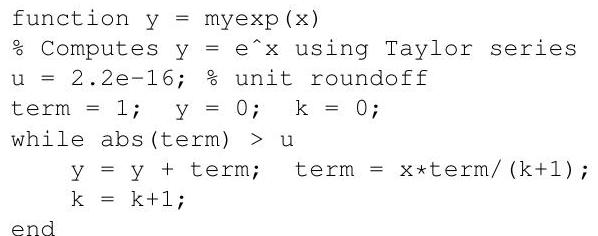
\includegraphics{2022_05_24_68a702cbf9a84fb58e04g-06}

This code gives accurate values for small $x$. But when $x=-20$ is used as the input, the computed value is $\approx 5.62 \times 10^{-9}$, while exp $(-20)$ gives $\approx 2.06 \times 10^{-9}$; there is not even one correct digit. Investigation shows that during the computation of myexp $(-20)$, the value of term becomes as large as $\approx 4.3 \times 10^{7}$. Use your knowledge of floating point arithmetic (in double precision) to explain why the error is so large. This appears to be a problem for large negative values of $x$. How can you modify this code to give accurate values for all $x$ (ignoring the problems of over- and underflow)?
%%%%%%%%%%%%%%%%%%%%%%%%%%%%%%%%%%%%%%%%%%%%%%%%%%%%%%%%%%%%%%%%%%%%%%%%%%%%%%%%%%%%%%%%%%%%%%%%%%%%%%%%%%%%%%%%%%%%%%%%
\newpage
%%%%%%%%%%%%%%%%%%%%%%%%%%%%%%%%%%%%%%%%%%%%%%%%%%%%%%%%%%%%%%%%%%%%%%%%%%%%%%%%%%%%%%%%%%%%%%%%%%%%%%%%%%%%%%%%%%%%%%%%
Write out formulas or pseudo-code for the Newton and secant methods for solving $f(x)=0$. List all conditions needed in order for these methods to converge. Give the expected rates of convergence of these methods under the conditions you have stated. Explain your terms. Perform three steps of Newton's method to find the positive root of $x^{3}-3 x-3=0$ using a starting value of $x_{0}=2$.
%%%%%%%%%%%%%%%%%%%%%%%%%%%%%%%%%%%%%%%%%%%%%%%%%%%%%%%%%%%%%%%%%%%%%%%%%%%%%%%%%%%%%%%%%%%%%%%%%%%%%%%%%%%%%%%%%%%%%%%%
\newpage
%%%%%%%%%%%%%%%%%%%%%%%%%%%%%%%%%%%%%%%%%%%%%%%%%%%%%%%%%%%%%%%%%%%%%%%%%%%%%%%%%%%%%%%%%%%%%%%%%%%%%%%%%%%%%%%%%%%%%%%%
Given a function $f(x)$ on an interval $[a, b]$ and points $a \leq x_{0}<x_{1}<x_{2}<$ $\cdots<x_{n} \leq b$, give a method to construct a polynomial $p(x)$ of degree $\leq n$ where $p$ interpolates $f$ at $x_{0}, x_{1}, \ldots, x_{n}$. (You do not have to give pseudocode, but it should be a clear and complete description.) Give a formula for estimating the interpolation error $f(x)-p(x)$. What is Chebyshev interpolation? From the formula for the interpolation error, explain how Chebyshev interpolation relates to minimax approximation.
%%%%%%%%%%%%%%%%%%%%%%%%%%%%%%%%%%%%%%%%%%%%%%%%%%%%%%%%%%%%%%%%%%%%%%%%%%%%%%%%%%%%%%%%%%%%%%%%%%%%%%%%%%%%%%%%%%%%%%%%
\newpage
%%%%%%%%%%%%%%%%%%%%%%%%%%%%%%%%%%%%%%%%%%%%%%%%%%%%%%%%%%%%%%%%%%%%%%%%%%%%%%%%%%%%%%%%%%%%%%%%%%%%%%%%%%%%%%%%%%%%%%%%
Consider solving the initial value problem $y^{\prime}=f(x, y)$ for $0 \leq x \leq 1$, $y(0)=Y_{0}, f$ being a smooth function. Let $0=x_{0}<x_{1}<\cdots<x_{N}=1$ be a uniform partition of the interval $[0,1]$ and denote $h$ the step size. Consider a method of the form
$$
\begin{aligned}
y_{n+1} &=\alpha y_{n}+\beta y_{n-1}+h \gamma f\left(x_{n-1}, y_{n-1}\right), \quad n \geq 1 \\
y_{0} &=Y_{0}, \quad y_{1}=Y_{0}+h f\left(x_{0}, Y_{0}\right)
\end{aligned}
$$
Choose the constants $\alpha, \beta$, and $\gamma$ so that the order of the method is as high as possible. Determine whether the resulting method is convergent.
%%%%%%%%%%%%%%%%%%%%%%%%%%%%%%%%%%%%%%%%%%%%%%%%%%%%%%%%%%%%%%%%%%%%%%%%%%%%%%%%%%%%%%%%%%%%%%%%%%%%%%%%%%%%%%%%%%%%%%%%
\newpage
%%%%%%%%%%%%%%%%%%%%%%%%%%%%%%%%%%%%%%%%%%%%%%%%%%%%%%%%%%%%%%%%%%%%%%%%%%%%%%%%%%%%%%%%%%%%%%%%%%%%%%%%%%%%%%%%%%%%%%%%
Define the Gauss-Jacobi method and the Gauss-Seidel method for solving the linear system $A \mathbf{x}=\mathbf{b}$, where $\mathbf{b} \in \mathbb{R}^{N}$ is given and
$$
A=\left(\begin{array}{ccccc}
2 & -1 & & & \\
-1 & 3 & -1 & & \\
& \ddots & \ddots & \ddots & \\
& & -1 & 3 & -1 \\
& & & -1 & 2
\end{array}\right) \in \mathbb{R}^{N \times N}
$$
For each method, determine a number of iterations to reduce the $\|\cdot\|_{\infty}$ norm of the error by a factor of $0.01$.
%%%%%%%%%%%%%%%%%%%%%%%%%%%%%%%%%%%%%%%%%%%%%%%%%%%%%%%%%%%%%%%%%%%%%%%%%%%%%%%%%%%%%%%%%%%%%%%%%%%%%%%%%%%%%%%%%%%%%%%%
\newpage
%%%%%%%%%%%%%%%%%%%%%%%%%%%%%%%%%%%%%%%%%%%%%%%%%%%%%%%%%%%%%%%%%%%%%%%%%%%%%%%%%%%%%%%%%%%%%%%%%%%%%%%%%%%%%%%%%%%%%%%%
What is the singular value decomposition (SVD) of a general rectangular matrix $A \in \mathbb{C}^{m \times n}$ ? For a $3 \times 3$ matrix $B$, compute $\|B\|_{2}$ and Cond $_{2}(B)=$ $\|B\|_{2}\left\|B^{-1}\right\|_{2}$ by taking advantage of the following SVD of the matrix $B$ (four significant digits after the decimal point are displayed):
$$
\begin{gathered}
\left(\begin{array}{rrr}
-0.3150 & -0.4193 & -0.8515 \\
-0.6449 & -0.5637 & 0.5161 \\
-0.6963 & 0.7117 & -0.0928
\end{array}\right)\left(\begin{array}{rrrr}
10.2377 & 0 & 0 \\
0 & 4.4830 & 0 \\
0 & 0 & 0.3050
\end{array}\right) \\
\times\left(\begin{array}{rrr}
-0.5598 & 0.3230 & 0.7630 \\
-0.7216 & 0.2625 & -0.6406 \\
-0.4073 & -0.9092 & 0.0861
\end{array}\right)
\end{gathered}
$$
%%%%%%%%%%%%%%%%%%%%%%%%%%%%%%%%%%%%%%%%%%%%%%%%%%%%%%%%%%%%%%%%%%%%%%%%%%%%%%%%%%%%%%%%%%%%%%%%%%%%%%%%%%%%%%%%%%%%%%%%
\newpage
%%%%%%%%%%%%%%%%%%%%%%%%%%%%%%%%%%%%%%%%%%%%%%%%%%%%%%%%%%%%%%%%%%%%%%%%%%%%%%%%%%%%%%%%%%%%%%%%%%%%%%%%%%%%%%%%%%%%%%%%
Give the Newton method for solving the equation
$$
e^{x}+4 e^{-x}-4=0
$$
and discuss the convergence order of the method. 2. Let $f(x)=\sin (\pi x)$.
%%%%%%%%%%%%%%%%%%%%%%%%%%%%%%%%%%%%%%%%%%%%%%%%%%%%%%%%%%%%%%%%%%%%%%%%%%%%%%%%%%%%%%%%%%%%%%%%%%%%%%%%%%%%%%%%%%%%%%%%
\newpage
%%%%%%%%%%%%%%%%%%%%%%%%%%%%%%%%%%%%%%%%%%%%%%%%%%%%%%%%%%%%%%%%%%%%%%%%%%%%%%%%%%%%%%%%%%%%%%%%%%%%%%%%%%%%%%%%%%%%%%%%
Determine a function $p(x)$ such that $p(x)$ is a polynomial on $[0,0.5]$ and $[0.5,1]$, and satisfies the conditions
$$
p(x)=f(x), p^{\prime}(x)=f^{\prime}(x), \quad \text { for } x=0,0.5,1
$$
%%%%%%%%%%%%%%%%%%%%%%%%%%%%%%%%%%%%%%%%%%%%%%%%%%%%%%%%%%%%%%%%%%%%%%%%%%%%%%%%%%%%%%%%%%%%%%%%%%%%%%%%%%%%%%%%%%%%%%%%
\newpage
%%%%%%%%%%%%%%%%%%%%%%%%%%%%%%%%%%%%%%%%%%%%%%%%%%%%%%%%%%%%%%%%%%%%%%%%%%%%%%%%%%%%%%%%%%%%%%%%%%%%%%%%%%%%%%%%%%%%%%%%
(a) Find $A_{0}, A_{1}$ and $A_{2}$ such that the integration rule
$$
I(f)=\int_{-h}^{h} f(x) d x \approx A_{0} f(-h / 2)+A_{1} f(0)+A_{2} f(h / 2)
$$
is exact for polynomials of degree $\leq 2$.
(b) Show that the rule constructed in $(\mathrm{a})$ is in fact exact for polynomials of degree $\leq 3$.

(c) For the constructed rule, it can be proved that
$$
I(f)-\left(A_{0} f(-h / 2)+A_{1} f(0)+A_{2} f(h / 2)\right)=c_{0} f^{(4)}(\eta) h^{5}, \quad \eta \in[-h, h]
$$
where $c_{0}$ is a constant independent of $f$. Find the constant $c_{0}$.
%%%%%%%%%%%%%%%%%%%%%%%%%%%%%%%%%%%%%%%%%%%%%%%%%%%%%%%%%%%%%%%%%%%%%%%%%%%%%%%%%%%%%%%%%%%%%%%%%%%%%%%%%%%%%%%%%%%%%%%%
\newpage
%%%%%%%%%%%%%%%%%%%%%%%%%%%%%%%%%%%%%%%%%%%%%%%%%%%%%%%%%%%%%%%%%%%%%%%%%%%%%%%%%%%%%%%%%%%%%%%%%%%%%%%%%%%%%%%%%%%%%%%%
4. Suppose that $B \approx A^{-1}$. Starting with an initial guess $x_{0}$, consider the following residual correction method:
$$
\begin{aligned}
&\text { for } k=0,1,2, \ldots \\
&r_{k} \longleftarrow A x_{k}-b \\
&x_{k+1} \leftarrow x_{k}-B r_{k}
\end{aligned}
$$
Show that this will converge (using exact arithmetic) so that $x_{k} \rightarrow x$, with $x$ the exact solution, provided $\|I-B A\|<1$.
%%%%%%%%%%%%%%%%%%%%%%%%%%%%%%%%%%%%%%%%%%%%%%%%%%%%%%%%%%%%%%%%%%%%%%%%%%%%%%%%%%%%%%%%%%%%%%%%%%%%%%%%%%%%%%%%%%%%%%%%
\newpage
%%%%%%%%%%%%%%%%%%%%%%%%%%%%%%%%%%%%%%%%%%%%%%%%%%%%%%%%%%%%%%%%%%%%%%%%%%%%%%%%%%%%%%%%%%%%%%%%%%%%%%%%%%%%%%%%%%%%%%%%
5. What is the QR factorization of a matrix? Explain how a QR factorization of a matrix can be computed using any of the following three methods: (i) Gram-Schmidt orthgonalization, (ii) Givens' rotations, or (iii) Householder reflectors.

An overdetermined linear system $A x=b$ where $A$ is $m \times n$ with $m>n$ usually cannot be solved for $x$. Instead we can ask to minimize $\|A x-b\|_{2}$ over all $x$. Show how the solution to this minimization problem can be computed using the QR factorization of $A$.
%%%%%%%%%%%%%%%%%%%%%%%%%%%%%%%%%%%%%%%%%%%%%%%%%%%%%%%%%%%%%%%%%%%%%%%%%%%%%%%%%%%%%%%%%%%%%%%%%%%%%%%%%%%%%%%%%%%%%%%%
\newpage
%%%%%%%%%%%%%%%%%%%%%%%%%%%%%%%%%%%%%%%%%%%%%%%%%%%%%%%%%%%%%%%%%%%%%%%%%%%%%%%%%%%%%%%%%%%%%%%%%%%%%%%%%%%%%%%%%%%%%%%%
6. Consider the following two methods for numerically solving an initial value problem for the $\mathrm{ODE} d x / d t=f(t, x)$ :
$$
\begin{aligned}
&x_{n+1}=x_{n-1}+2 h f\left(t_{n}, x_{n}\right) \quad \text { (leap-frog method) } \\
&x_{n+1}=x_{n}+(h / 2)\left[f\left(t_{n}, x_{n}\right)+f\left(t_{n+1}, x_{n+1}\right)\right] \quad \text { (implicit mid-point method) }
\end{aligned}
$$
where $h$ is the step size, and $t_{k}=t_{0}+k h$. For the test equation $d x / d t=\lambda x$, show that the leap-frog method is only stable for $\lambda h=0$, while the implicit mid-point method is stable for all $\lambda h<0$.
%%%%%%%%%%%%%%%%%%%%%%%%%%%%%%%%%%%%%%%%%%%%%%%%%%%%%%%%%%%%%%%%%%%%%%%%%%%%%%%%%%%%%%%%%%%%%%%%%%%%%%%%%%%%%%%%%%%%%%%%
\newpage
%%%%%%%%%%%%%%%%%%%%%%%%%%%%%%%%%%%%%%%%%%%%%%%%%%%%%%%%%%%%%%%%%%%%%%%%%%%%%%%%%%%%%%%%%%%%%%%%%%%%%%%%%%%%%%%%%%%%%%%%
Floating point arithmetic. In Matlab, the formulas
$$
\begin{aligned}
\cos \theta &=\frac{x}{\sqrt{x^{2}+y^{2}}} \\
\sin \theta &=\frac{y}{\sqrt{x^{2}+y^{2}}}
\end{aligned}
$$
give $\cos \theta=\sin \theta=0$ for $x=y=10^{+200}$. Why does this occur? Can you re-arrange the formulas to give equivalent formulas in exact arithmetic, but give accurate values for $\cos \theta$ and $\sin \theta$.
%%%%%%%%%%%%%%%%%%%%%%%%%%%%%%%%%%%%%%%%%%%%%%%%%%%%%%%%%%%%%%%%%%%%%%%%%%%%%%%%%%%%%%%%%%%%%%%%%%%%%%%%%%%%%%%%%%%%%%%%
\newpage
%%%%%%%%%%%%%%%%%%%%%%%%%%%%%%%%%%%%%%%%%%%%%%%%%%%%%%%%%%%%%%%%%%%%%%%%%%%%%%%%%%%%%%%%%%%%%%%%%%%%%%%%%%%%%%%%%%%%%%%%
Solution of nonlinear equations. Carry out two steps of the secant method for solving $x e^{x}=3$ starting with $x_{0}=0$ and $x_{1}=1$. What rate of convergence is expected, and under what conditions is this rate of convergence obtained?
%%%%%%%%%%%%%%%%%%%%%%%%%%%%%%%%%%%%%%%%%%%%%%%%%%%%%%%%%%%%%%%%%%%%%%%%%%%%%%%%%%%%%%%%%%%%%%%%%%%%%%%%%%%%%%%%%%%%%%%%
\newpage
%%%%%%%%%%%%%%%%%%%%%%%%%%%%%%%%%%%%%%%%%%%%%%%%%%%%%%%%%%%%%%%%%%%%%%%%%%%%%%%%%%%%%%%%%%%%%%%%%%%%%%%%%%%%%%%%%%%%%%%%
Interpolation and approximation. Using equally spaced interpolation points is known to result in Runge's phenomenon for the function $f(x)=1 /\left(1+x^{2}\right)$ interpolated over $[-5,+5]$. What is this phenomenon? Can the use of a different set of interpolation points prevent this phenomenon? If so, explain how?
%%%%%%%%%%%%%%%%%%%%%%%%%%%%%%%%%%%%%%%%%%%%%%%%%%%%%%%%%%%%%%%%%%%%%%%%%%%%%%%%%%%%%%%%%%%%%%%%%%%%%%%%%%%%%%%%%%%%%%%%
\newpage
%%%%%%%%%%%%%%%%%%%%%%%%%%%%%%%%%%%%%%%%%%%%%%%%%%%%%%%%%%%%%%%%%%%%%%%%%%%%%%%%%%%%%%%%%%%%%%%%%%%%%%%%%%%%%%%%%%%%%%%%
 Numerical integration. Use Simpson's method with five function evaluations to obtain an estimate of $\int_{0}^{1} e^{x} /(1+x) d x$. What is the asymptotic order of the error of composite Simpson's method with $2 n+1$ function evaluations? Give an example of a method that has an asymptotically faster rate of convergence than Simpson's method as the number of function evaluations goes to infinity.
%%%%%%%%%%%%%%%%%%%%%%%%%%%%%%%%%%%%%%%%%%%%%%%%%%%%%%%%%%%%%%%%%%%%%%%%%%%%%%%%%%%%%%%%%%%%%%%%%%%%%%%%%%%%%%%%%%%%%%%%
\newpage
%%%%%%%%%%%%%%%%%%%%%%%%%%%%%%%%%%%%%%%%%%%%%%%%%%%%%%%%%%%%%%%%%%%%%%%%%%%%%%%%%%%%%%%%%%%%%%%%%%%%%%%%%%%%%%%%%%%%%%%%
 Multistep methods. Consider the general multistep method
$$
\begin{aligned}
y_{n+1} &=\sum_{j=0}^{p} a_{j} y_{n-j}+h \sum_{j=-1}^{p} b_{j} f\left(t_{n-j}, y_{n-j}\right) \\
&=\sum_{j=0}^{p} a_{j} y_{n-j}+h \sum_{j=-1}^{p} b_{j} y_{n-j}^{\prime} .
\end{aligned}
$$
In order to prove convergence of a particular order for this method we need two basic conditions: a stability condition, and a consistency condition. [Hint: The consistency conditions come from Taylor series expansions of $\boldsymbol{y}_{n-j}=\boldsymbol{y}\left(t_{n-j}\right)$. Give these conditions. Use them to determine if, and with what order, the trapezoidal method converges:
$$
y_{n+1}=y_{n-1}+\frac{h}{2}\left[f\left(t_{n}, y_{n}\right)+f\left(t_{n+1}, y_{n+1}\right)\right] .
$$
Correction: $y_{n-1}$ on the right should be $y_{n}$.
$$
y_{n+1}=y_{n}+\frac{h}{2}\left[f\left(t_{n}, y_{n}\right)+f\left(t_{n+1}, y_{n+1}\right)\right] .
$$

End of correction.
%%%%%%%%%%%%%%%%%%%%%%%%%%%%%%%%%%%%%%%%%%%%%%%%%%%%%%%%%%%%%%%%%%%%%%%%%%%%%%%%%%%%%%%%%%%%%%%%%%%%%%%%%%%%%%%%%%%%%%%%
\newpage
%%%%%%%%%%%%%%%%%%%%%%%%%%%%%%%%%%%%%%%%%%%%%%%%%%%%%%%%%%%%%%%%%%%%%%%%%%%%%%%%%%%%%%%%%%%%%%%%%%%%%%%%%%%%%%%%%%%%%%%%
Runge-Kutta methods. Show that Heun's method
$$
\begin{aligned}
\mathbf{z}_{n+1} &=\mathbf{y}_{n}+h \mathbf{f}\left(t_{n}, \mathbf{y}_{n}\right) \\
\mathbf{y}_{n+1} &=\mathbf{y}_{n}+\frac{1}{2} h\left[\mathbf{f}\left(t_{n}, \mathbf{y}_{n}\right)+\mathbf{f}\left(t_{n+1}, \mathbf{z}_{n+1}\right)\right]
\end{aligned}
$$
has a local truncation error of $\mathcal{O}\left(h^{3}\right)$. What is its asymptotic global truncation error in the form $\mathcal{O}\left(h^{m}\right)$ ?
%%%%%%%%%%%%%%%%%%%%%%%%%%%%%%%%%%%%%%%%%%%%%%%%%%%%%%%%%%%%%%%%%%%%%%%%%%%%%%%%%%%%%%%%%%%%%%%%%%%%%%%%%%%%%%%%%%%%%%%%
\newpage
%%%%%%%%%%%%%%%%%%%%%%%%%%%%%%%%%%%%%%%%%%%%%%%%%%%%%%%%%%%%%%%%%%%%%%%%%%%%%%%%%%%%%%%%%%%%%%%%%%%%%%%%%%%%%%%%%%%%%%%%
LU factorization and linear systems. The perturbation theorem for linear systems states that if $A \boldsymbol{x}=\boldsymbol{b},(A+E) \widehat{x}=\boldsymbol{b}+\boldsymbol{d}$, and $\left\|A^{-1}\right\|\|E\|<$ 1 , then
$$
\frac{\|\widehat{x}-x\|}{\|x\|} \leq \frac{\kappa(A)}{1-\kappa(A)(\|E\| /\|A\|)}\left[\frac{\|E\|}{\|A\|}+\frac{\|\boldsymbol{d}\|}{\|\boldsymbol{b}\|}\right]
$$
where $\kappa(A)=\left\|A^{-1}\right\|\|A\|$ is the condition number. Using this, how many digits of accuracy are expected in the computed solution $\hat{x}$ given that the matrix $A$ and right-hand side $b$ are known to 5 digits, but $\kappa(A) \approx 10^{3}$ ? The backward error theory for $L U$ factorization by Wilkinson shows that the computed solution $\widehat{x}$ of a system $A x=\boldsymbol{b}$ exactly satisfies $(A+E) \widehat{x}=\boldsymbol{b}$ where $\|E\|_{\infty} \leq 3 \mathbf{u}\left(\|A\|_{\infty}+\|\widehat{L}\|_{\infty}\|\widehat{U}\|_{\infty}\right)$ Where $\hat{L}$ and $\widehat{U}$ are the computed $L$ and $U$ factors in the $L U$ factorization. If $\|\widehat{L}\|_{\infty}\|\widehat{U}\|_{\infty} /\|A\|_{\infty}$ is modest (say $\left.\approx 10\right)$, give an estimate for the relative error $\|\widehat{x}-x\|_{\infty} /\|x\|_{\infty}$ in terms of $\kappa(A)$ in the $\infty-$ norm.
%%%%%%%%%%%%%%%%%%%%%%%%%%%%%%%%%%%%%%%%%%%%%%%%%%%%%%%%%%%%%%%%%%%%%%%%%%%%%%%%%%%%%%%%%%%%%%%%%%%%%%%%%%%%%%%%%%%%%%%%
\newpage
%%%%%%%%%%%%%%%%%%%%%%%%%%%%%%%%%%%%%%%%%%%%%%%%%%%%%%%%%%%%%%%%%%%%%%%%%%%%%%%%%%%%%%%%%%%%%%%%%%%%%%%%%%%%%%%%%%%%%%%%
$Q R$ algorithm. Give the $Q R$ algorithm (with or without shifting). Show that if the original matrix $A$ is symmetric, then every iterate of the QR factorization is symmetric. Explain how shifting is used to improve the rate of convergence of the QR algorithm.
%%%%%%%%%%%%%%%%%%%%%%%%%%%%%%%%%%%%%%%%%%%%%%%%%%%%%%%%%%%%%%%%%%%%%%%%%%%%%%%%%%%%%%%%%%%%%%%%%%%%%%%%%%%%%%%%%%%%%%%%
\newpage
%%%%%%%%%%%%%%%%%%%%%%%%%%%%%%%%%%%%%%%%%%%%%%%%%%%%%%%%%%%%%%%%%%%%%%%%%%%%%%%%%%%%%%%%%%%%%%%%%%%%%%%%%%%%%%%%%%%%%%%%
Multistep methods. Consider the general multistep method
$$
y_{n+1}=\sum_{j=0}^{p} a_{j} y_{n-j}+h \sum_{j=-1}^{p} b_{j} f\left(t_{n-j}, y_{n-j}\right) .
$$
In order to prove convergence of a particular order for this method we need two basic conditions: a stability condition, and a consistency condition. Give these conditions. Use them to determine if, and with what order, the leap-frog method converges:
$$
y_{n+1}=y_{n-1}+2 h f\left(t_{n}, y_{n}\right) .
$$
%%%%%%%%%%%%%%%%%%%%%%%%%%%%%%%%%%%%%%%%%%%%%%%%%%%%%%%%%%%%%%%%%%%%%%%%%%%%%%%%%%%%%%%%%%%%%%%%%%%%%%%%%%%%%%%%%%%%%%%%
\newpage
%%%%%%%%%%%%%%%%%%%%%%%%%%%%%%%%%%%%%%%%%%%%%%%%%%%%%%%%%%%%%%%%%%%%%%%%%%%%%%%%%%%%%%%%%%%%%%%%%%%%%%%%%%%%%%%%%%%%%%%%
Runge-Kutta methods. The implicit trapezoidal rule is
$$
y_{n+1}=y_{n}+\frac{1}{2} h\left[f\left(t_{n}, y_{n}\right)+f\left(t_{n+1}, y_{n+1}\right)\right] .
$$
Describe what is meant by the stability region of a Runge-Kutta method. What is the stability region for the implicit trapezoidal method? Rigorously justify your answer.
%%%%%%%%%%%%%%%%%%%%%%%%%%%%%%%%%%%%%%%%%%%%%%%%%%%%%%%%%%%%%%%%%%%%%%%%%%%%%%%%%%%%%%%%%%%%%%%%%%%%%%%%%%%%%%%%%%%%%%%%
\newpage
%%%%%%%%%%%%%%%%%%%%%%%%%%%%%%%%%%%%%%%%%%%%%%%%%%%%%%%%%%%%%%%%%%%%%%%%%%%%%%%%%%%%%%%%%%%%%%%%%%%%%%%%%%%%%%%%%%%%%%%%
$L U$ factorization and linear systems. The perturbation theorem for linear systems states that if $A x=b,(A+E) \widehat{x}=b+d$, and $\left\|A^{-1}\right\|\|E\|<1$, then
$$
\frac{\|\widehat{x}-x\|}{\|x\|} \leq \frac{\kappa(A)}{1-\kappa(A)(\|E\| /\|A\|)}\left[\frac{\|E\|}{\|A\|}+\frac{\|d\|}{\|b\|}\right]
$$
where $\kappa(A)=\left\|A^{-1}\right\|\|A\|$ is the condition number. Using this, how many digits of accuracy are expected in the computed solution $\hat{x}$ given that the matrix $A$ and right-hand side $b$ are known to 5 digits, but $\kappa(A) \approx 10^{3}$ ? The backward error theory for $L U$ factorization by Wilkinson shows that the computed solution $\hat{x}$ of a system $A x=b$ exactly satisfies $(A+E) \widehat{x}=b$ where $\|E\|_{\infty} \leq 3 \mathbf{u}\left(\|A\|_{\infty}+\|\widehat{L}\|_{\infty}\|\widehat{U}\|_{\infty}\right)$ where $\widehat{L}$ and $\widehat{U}$ are the computed $L$ and $U$ factors in the $L U$ factorization. If $\|\widehat{L}\|_{\infty}\|\widehat{U}\|_{\infty} /\|A\|_{\infty}$ is modest $($ say $\approx 10)$, give an estimate for the relative error $\|\widehat{x}-x\|_{\infty} /\|x\|_{\infty}$ in terms of $\kappa(A)$ in the $\infty$-norm.
%%%%%%%%%%%%%%%%%%%%%%%%%%%%%%%%%%%%%%%%%%%%%%%%%%%%%%%%%%%%%%%%%%%%%%%%%%%%%%%%%%%%%%%%%%%%%%%%%%%%%%%%%%%%%%%%%%%%%%%%
\newpage
%%%%%%%%%%%%%%%%%%%%%%%%%%%%%%%%%%%%%%%%%%%%%%%%%%%%%%%%%%%%%%%%%%%%%%%%%%%%%%%%%%%%%%%%%%%%%%%%%%%%%%%%%%%%%%%%%%%%%%%%
Least squares, Cholesky and $Q R$ factorization. The normal equations for solving a least squares problem $\min _{x}\|A x-b\|_{2}$ are $A^{T} A x=A^{T} b$. Describe precisely what the Cholesky and $Q R$ factorizations are. Show how to solve the least squares problem using either the $Q R$ factorization applied to the original system, or Cholesky factorization applied to the normal equations for the least squares problem. Also show that the $R$ matrix in the $Q R$ factorization of $A$ is one of the factors in a Cholesky factorization of $A^{T} A$.
%%%%%%%%%%%%%%%%%%%%%%%%%%%%%%%%%%%%%%%%%%%%%%%%%%%%%%%%%%%%%%%%%%%%%%%%%%%%%%%%%%%%%%%%%%%%%%%%%%%%%%%%%%%%%%%%%%%%%%%%
\newpage
%%%%%%%%%%%%%%%%%%%%%%%%%%%%%%%%%%%%%%%%%%%%%%%%%%%%%%%%%%%%%%%%%%%%%%%%%%%%%%%%%%%%%%%%%%%%%%%%%%%%%%%%%%%%%%%%%%%%%%%%
\end{document}